

%% this section contains XX problems
%%----------------------------------------


%% Jacobs 5 steps to a 5
%%------------------------------
\element{AP}{
\begin{question}{Jacobs-Q14}
    A mass on a spring has a frequency of \SI{2.5}{\hertz}
        and an amplitude of \SI{0.05}{\meter}.
    What is the period of the oscillations?
    \begin{multicols}{2}
    \begin{choices}
      \correctchoice{\SI{0.4}{\second}}
        \wrongchoice{\SI{0.2}{\second}}
        \wrongchoice{\SI{8}{\second}}
        \wrongchoice{\SI{20}{\second}}
        \wrongchoice{\SI{50}{\second}}
    \end{choices}
    \end{multicols}
\end{question}
}

\element{AP}{
\begin{question}{Jacobs-Q15}
    A mass $m$ oscillates on a horizontal spring of
        constant $k$ with no damping.
    The amplitude of the oscillation is $A$.
    What is the potential energy of the mass
        at its maximum displacement?
    \begin{multicols}{2}
    \begin{choices}
        \wrongchoice{zero}
        \wrongchoice{$mgh$}
        \wrongchoice{$kA$}
        \wrongchoice{$\frac{1}{2}mv^2$}
      \correctchoice{$\frac{1}{2}kA^2$}
    \end{choices}
    \end{multicols}
\end{question}
}

\element{AP}{
\begin{question}{Jacobs-APB-Q14}
    Block $B$ is at rest on a smooth tabletop.
    It is attached to a long spring, which in turn
        is anchored to the wall.
    Block $A$ slides toward and collides with block $B$.
    \begin{center}
        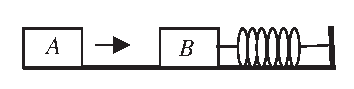
\includegraphics[keepaspectratio,scale=0.5]{Jacobs-APB-Q14}
    \end{center}
    Consider two possible collisions:
    \begin{itemize}
        \item[Case I:] block $A$ bounces back off of block $B$
        \item[Case II:] block $A$ sticks to block $B$.
    \end{itemize}
    Which of the following is correct about the speed of block $B$
        immediateyl after the collision?
    \begin{choices}
        \wrongchoice{It is faster in case II than in case I \emph{only} if block $B$ is heavier.}
        \wrongchoice{It is faster in case I than in case II \emph{only} if block $B$ is heavier.}
        \wrongchoice{It is faster in case II than in case I regardless of the mass
                of each block.}
      \correctchoice{It is faster in case I than in case II regardless of the mass
                of each block.}
        \wrongchoice{It is the same in either case regardless of the mass
                of each block.}
    \end{choices}
\end{question}
}

\element{AP}{
\begin{question}{Jacobs-APB-Q15}
    Block $B$ is at rest on a smooth tabletop.
    It is attached to a long spring, which in turn
        is anchored to the wall.
    Block $A$ slides toward and collides with block $B$.
    \begin{center}
        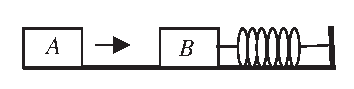
\includegraphics[keepaspectratio,scale=0.5]{Jacobs-APB-Q14}
    \end{center}
    Consider two possible collisions:
    \begin{itemize}
        \item[Case I:] block $A$ bounces back off of block $B$
        \item[Case II:] block $A$ sticks to block $B$.
    \end{itemize}
    Which is correct about the period of the ensuing oscillations after
        the collision?
    \begin{choices}
        \wrongchoice{The period is greater in case II than in case I if block $B$ is heavier.}
        \wrongchoice{The period is greater in case I than in case II if block $B$ is heavier.}
      \correctchoice{The period is greater in case II than in case I
            regardless of the mass of each block.}
        \wrongchoice{The period is greater in case I than in case II
            regardless of the mass of each block.}
        \wrongchoice{The period is the same in either case.}
    \end{choices}
\end{question}
}

\element{AP}{
\begin{question}{Jacobs-APB-Q21}
    A ball of mass $m$ on a string swings back and forth to
        a maximum angle of \ang{30} to the vertical, as shown below.
    \begin{center}
        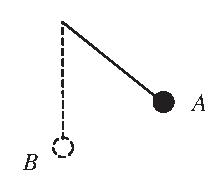
\includegraphics[keepaspectratio,scale=0.5]{Jacobs-APB-Q21}
    \end{center}
    Which of the following vectors represents the acceleration,
        $a$, of the mass at point $A$, the highest point in the swing?
    \begin{choices}
        \wrongchoice{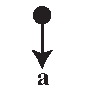
\includegraphics[keepaspectratio,scale=0.5]{Jacobs-APB-Q21-A}}
        \wrongchoice{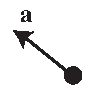
\includegraphics[keepaspectratio,scale=0.5]{Jacobs-APB-Q21-B}}
      \correctchoice{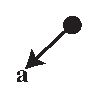
\includegraphics[keepaspectratio,scale=0.5]{Jacobs-APB-Q21-C}}
        \wrongchoice{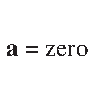
\includegraphics[keepaspectratio,scale=0.5]{Jacobs-APB-Q21-D}}
        \wrongchoice{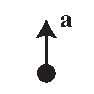
\includegraphics[keepaspectratio,scale=0.5]{Jacobs-APB-Q21-E}}
    \end{choices}
\end{question}
}

\element{AP}{
\begin{question}{Jacobs-APB-Q53}
    A guitar string is plucked, producing a standing wave on the
        string.
    A person hears the sound wave generated by the string.
    Which wave properties are the same for each of these wave,
        and which are different?
    \begin{multicols}{3}
    \begin{choices}
        \wrongchoice{$3 \lambda$}
        \wrongchoice{$2 \lambda$}
        \wrongchoice{$\lambda$}
        \wroonghoice{$\dfrac{\lambda}{2}$}
      \correctchoice{$\dfrac{\lambda}{4}$}
    \end{choices}
    \end{multicols}
\end{question}
}


%% 2004-APB
%%------------------------------
\element{AP}{
\begin{question}{2004-APB-Q01}
    For which of the following motions of an object must
        the acceleration always be zero?
    \begin{itemize}
        \item[I.] Any motion in a straight line
        \item[I.] Simple harmonic motion
        \item[I.] Any motion in a circle
    \end{itemize}
    \begin{multicols}{2}
    \begin{choices}
      \correctchoice{I only}
        \wrongchoice{II only}
        \wrongchoice{III only}
        \wrongchoice{Either I or III, but not II}
        \wrongchoice{None of these motions guarantees zero acceleration}
    \end{choices}
    \end{multicols}
\end{question}
}

\element{AP}{
\begin{question}{2004-APB-Q07}
    A sphere of mass $m_1$, which is attached to a spring, is displaced
        downward from it equilibrium position as shown above left and
        released from rest.
    A sphere of mass $m_2$, which is suspended from a string of length $l$,
        is displaced to the right as shown above right and released from
        rest so that it swings as a simple pendulum with small amplitude.
    Assume that both spheres undergo simple harmonic motion.
    \begin{center}
        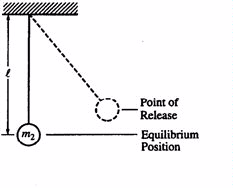
\includegraphics[keepaspectratio]{2004-APB-Q06-left}
        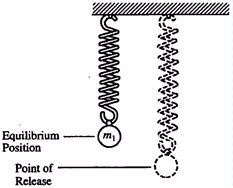
\includegraphics[keepaspectratio]{2004-APB-Q06-right}
    \end{center}
    If both both spheres have the same period of oscillation,
        which of the following is an expression for the spring constant?
    \begin{choices}
        \wrongchoice{$\dfrac{l}{m_1 g}$}
        \wrongchoice{$\dfrac{g}{m_2 l}$}
        \wrongchoice{$\dfrac{m_1}{g}$}
        \wrongchoice{$\dfrac{m_2 g}{l}$}
      \correctchoice{$\dfrac{m_1 g}{l}$}
    \end{choices}
\end{question}
}

\element{AP}{
\begin{question}{2004-APB-Q08}
    A block attached to the lower end of a vertical spring oscillates up
        and down.
    If the spring obeys Hooke's law, the period of oscillation depends on
        which of the following?
    \begin{itemize}
        \item[I] Mass of the block
        \item[II] Amplitude of the oscillation
        \item[III] Force constant of the spring
    \end{itemize}
    \begin{choices}
        \wrongchoice{I, only}
        \wrongchoice{II, only}
        \wrongchoice{III, only}
      \correctchoice{I and II, only}
        \wrongchoice{I and III, only}
    \end{choices}
\end{question}
}

\element{AP}{
\begin{question}{2004-APB-Q43}
    A simple pendulum and a mass hanging on a spring both have
        a period of \SI{1}{\second} when set into small oscillatory
        motion on Earth.
    They are taken to planet $X$, which has the same diameter as
        Earth but twice the mass.
    Which of the following statements is true about the periods of
        the two objects on planet $X$ compared to their periods
        on Earth?
    \begin{choices}
        \wrongchoice{Both are shorter}
        \wrongchoice{Both are the same}
        \wrongchoice{Both are longer}
        \wrongchoice{The period of the mass on the spring is shorter, that of the pendulum is the same.}
      \correctchoice{The period of the pendulum is shorter, that of the mass on the spring is the same.}
    \end{choices}
\end{question}
}


